\chapter[High-level Design]{High-Level Design}

The overall design and architecture of the proposed system are presented here. A high-level representation of the system structure, major modules, component interactions, and data flow within the system is provided. The High-Level Design (HLD) phase transforms the requirements specified in Chapter 3 into a conceptual blueprint that guides the implementation process. System organisation, architecture strategies, module interactions, and workflow representation are focused upon without going into implementation-level or database-level details.


\section[Design Considerations]{Design Considerations}
This section explains the important factors considered while designing the proposed system. The purpose of this section is to justify the architectural, procedural, and design decisions taken during system planning. These factors ensure that the software remains robust, efficient, and user-friendly under variable operational conditions.
\subsection[General Considerations]{General Considerations}

Here are the general design factors rewritten as prescriptive principles and requirements considered during system development:

\subsubsection{System Scalability}
\begin{itemize}
    \item \textbf{Independent Scalability:} The frontend visualization layer and the backend optimization engine must be decoupled to allow independent scaling under variable user loads.
    \item \textbf{Component-Level Extensibility:} The system architecture must support the addition of new logical nodes, pathways, or specialized agents without requiring changes to the core routing algorithms.
    \item \textbf{Adjacency-Based Network Expansion:} The network model must use flexible data structures so that the supply chain topology can grow without rewriting the backend codebase.
\end{itemize}

\subsubsection{Reliability}
\begin{itemize}
    \item \textbf{Deterministic Fallback Protocols:} The system must incorporate automatic fallback logic (such as mathematical overrides) to guarantee a valid routing decision even if external cognitive APIs experience downtime or high latency.
    \item \textbf{State Isolation:} The database and tracking metrics must run with strict session isolation to prevent state leakage and ensure execution results are reproducible.
\end{itemize}

\subsubsection{Maintainability}
\begin{itemize}
    \item \textbf{Separation of Concerns:} Core system configurations (such as physical network topologies and mapping rule libraries) must be isolated from the source code, utilizing external data files (like JSON) to simplify updates.
    \item \textbf{Modular Codebase:} Code structures must be organized into logical packages with distinct folders for routing engines, API endpoints, and benchmark scripts.
\end{itemize}

\subsubsection{Security}
\begin{itemize}
    \item \textbf{Credential Isolation:} The storage of third-party API keys and server credentials must be restricted to local environment files rather than hardcoded in the codebase.
    \item \textbf{Access Control \& Sandboxing:} Cognitive agents must operate with restricted permissions, modifying system variables or accessing database records only through structured, predefined interfaces.
\end{itemize}

\subsubsection{User-Friendliness}
\begin{itemize}
    \item \textbf{Geospatial \& Visual Simplification:} Complex textual routes and network logs must be represented as interactive, spatial visual pathways.
    \item \textbf{Consolidated Telemetry:} Key operational metrics (such as delays, financial deltas, and inventory warnings) must be displayed via clear, intuitive visual widgets.
\end{itemize}

\subsubsection{Performance Efficiency}
\begin{itemize}
    \item \textbf{Low-Latency Calculations:} Graph-theoretic and mathematical routing calculations must operate in-memory to ensure response times remain in milliseconds.
    \item \textbf{Minimal Payload Overheads:} Context passed to external reasoning APIs must be token-optimized to minimize latency and call costs.
\end{itemize}

\subsubsection{Modularity}
\begin{itemize}
    \item \textbf{Phase-Based Architecture:} The project pipeline must be divided into separate, independent modules for signal extraction, agentic orchestration, and mathematical execution so that each phase can be tested and modified in isolation.
\end{itemize}

\subsubsection{Reusability}
\begin{itemize}
    \item \textbf{Interface Standardization:} Functions, utilities, and components must be generic and reusable across different simulation scenarios.
\end{itemize}

\subsubsection{Flexibility}
\begin{itemize}
    \item \textbf{Dynamic Parameter Customization:} The system must allow users to toggle operational priorities (such as cost vs. time) and adjust simulation parameters dynamically during execution.
\end{itemize}
\subsection[Development Methods]{Development Methods}
This subsection explains the software development methodology adopted for the project. The project follows a 6-week sequential execution timeline, divided into five core modules. Each module corresponds directly to a layer in the system architecture.

Given the deeply interconnected nature of the system components and the requirement for a stable mathematical baseline, the project utilizes a \textbf{Sequential "Waterfall" Handover Strategy}. This model was selected to ensure that each critical layer of the logistics digital twin—from network topology to agentic reasoning—is rigorously validated and "frozen" before downstream logic is applied. This prevents cascading errors in the mathematical optimization engine.

The development methodology is divided into the following phases:

\begin{itemize}
    \item \textbf{Phase 1: Digital Twin Construction (Week 1)}: Mapping global maritime nodes to domestic SME hubs using \texttt{networkx}; establishing baseline edge weights such as transit time and logistics cost.
    \item \textbf{Phase 2: Domain Logic \& Data Generation (Week 2)}: Quantifying "Grey Zone" friction variables (insurance spikes, port delays) and building the Semantic Mapping Library to link geopolitical keywords to specific graph nodes.
    \item \textbf{Phase 3: Agentic Intelligence \& Monitoring (Week 3)}: Developing the \textit{Friction Sentry Agent} using LangChain and CrewAI to autonomously ingest unstructured news data and extract critical location and severity metrics.
    \item \textbf{Phase 4: Autonomous Mitigation \& Execution (Weeks 4--5)}: Developing the \textit{Logistics Optimizer Agent}; injecting friction shocks into the graph and executing shortest-path algorithms (Dijkstra's) to calculate optimal rerouting and dynamic buffer stocks.
    \item \textbf{Phase 5: Visualization \& Baseline Validation (Week 6)}: Calculating the "Human Baseline" using Chopra inventory formulas and deploying an interactive dashboard to visualize AI cost-savings versus manual planning.
\end{itemize}

To manage this sequential flow effectively within a decoupled architecture, the team adheres to an \textbf{Immutable Handover Protocol}, where each module must pass unit-testing before being consumed by the next:
\begin{itemize}
    \item \textbf{Network to AI (M1 to M3 \& M2)}: The Network Architect hands over the finalized logistics graph, which serves as the immutable environment for all agents.
    \item \textbf{Domain to Monitoring (M3 to M2)}: The Domain Specialist hands over the Semantic Dictionary; the AI Engineer cannot finalize the parsing agent until keyword mappings are locked.
    \item \textbf{Monitoring to Visualization (M2 to M4)}: The AI Engineer passes the final validated JSON payloads to the Dashboard Analyst for front-end integration.
\end{itemize}
\section[Architecture Strategies]{Architecture Strategies}
This section explains the architectural and technological strategies adopted during system design. Selecting the appropriate programming paradigms and technology stacks is essential to support high-performance operations research and cognitive reasoning. The logic behind choosing specific backend, frontend, and integration frameworks is elaborated below.

\subsection[Programming Language]{Programming Language}
The system utilizes a split-stack architecture, leveraging Python for the backend logic and React (JavaScript/ES6+) for the frontend visualization dashboard.

\subsubsection{Python (Backend \& Agentic Engine)}
Python was selected as the core engine due to its dominance in Artificial Intelligence and operations research. It provides a seamless bridge between cognitive AI frameworks (CrewAI, LangChain) and scientific computing libraries (NetworkX). Its high-level syntax and asynchronous capabilities via FastAPI allow for rapid prototyping of complex multi-agent workflows and real-time graph optimization.

\subsubsection{React \& JavaScript (Frontend Dashboard)}
React is employed to build the interactive User Interface. For a logistics digital twin, real-time telemetry and dynamic geospatial rendering are critical. React’s component-based architecture and Virtual DOM enable efficient updates of complex map visualizations (via React-Leaflet) and performance metrics without full page reloads, ensuring a responsive user experience during simulation shocks.

\subsection[Future Plans and Scalability]{Future Plans and Scalability}
This subsection outlines the strategic roadmap for evolving the system from a high-fidelity prototype to a production-grade autonomous logistics engine.

\subsubsection{Transition to Real-Time Data Pipelines}
While the current framework demonstrates autonomous reasoning on simulated or static historical data, future iterations will integrate \textbf{Live Telemetry Ingestion}. By connecting the \textit{Friction Sentry Agent} to real-time APIs (e.g., Lloyds List for maritime news, port congestion trackers, and satellite Automatic Identification System (AIS) data), the system will move from manual simulation to a "Live Sentry" mode, providing under-60-minute detection-to-mitigation cycles for Exim logistics.

\subsubsection{Multi-Dimensional Friction Modeling}
The architecture is designed to scale from single-point shocks to \textbf{Compound Risk Scenarios}. Future enhancements will focus on the agent's ability to process and correlate multiple simultaneous friction signals—such as a geopolitical blockade in a chokepoint occurring concurrently with a domestic labor strike. This involves developing cross-impact matrices where agents reason about how separate shocks propagate through the network and amplify total logistics cost.

\subsubsection{Predictive "Friction Forecasting"}
Leveraging the data captured during the current implementation, future versions could incorporate \textbf{Predictive Analytics Engines}. By training machine learning models on historical friction patterns, the system could transition from being reactive (mitigating current shocks) to proactive (recommending route adjustments based on high-probability future disruptions).

\subsubsection{Cloud-Native Enterprise Scaling}
To handle global-scale supply chains with thousands of nodes, the system can be migrated to a \textbf{Kubernetes-based Microservices Architecture}. This would allow the agentic swarm to scale horizontally, assigning dedicated agent clusters to specific geographic regions or product categories, ensuring low-latency optimization for multi-national logistics networks.

\section[System Architecture]{System Architecture}
This section explains the overall architecture and structural organization of the proposed system. A layered block layout is utilized to segregate the presentation, API routing, network optimization, and multi-agent reasoning layers. This division ensures that each component can be developed, tested, and scaled independently.

\subsection[High-Level Design Diagram]{High-Level Design Diagram}
The High-Level Design (HLD) diagram as shown in Figure \ref{fig:hldd} illustrates the multi-layered flow of information through the system, from raw data ingestion to final executive visualization.

\begin{figure}[htbp]
    \centering
    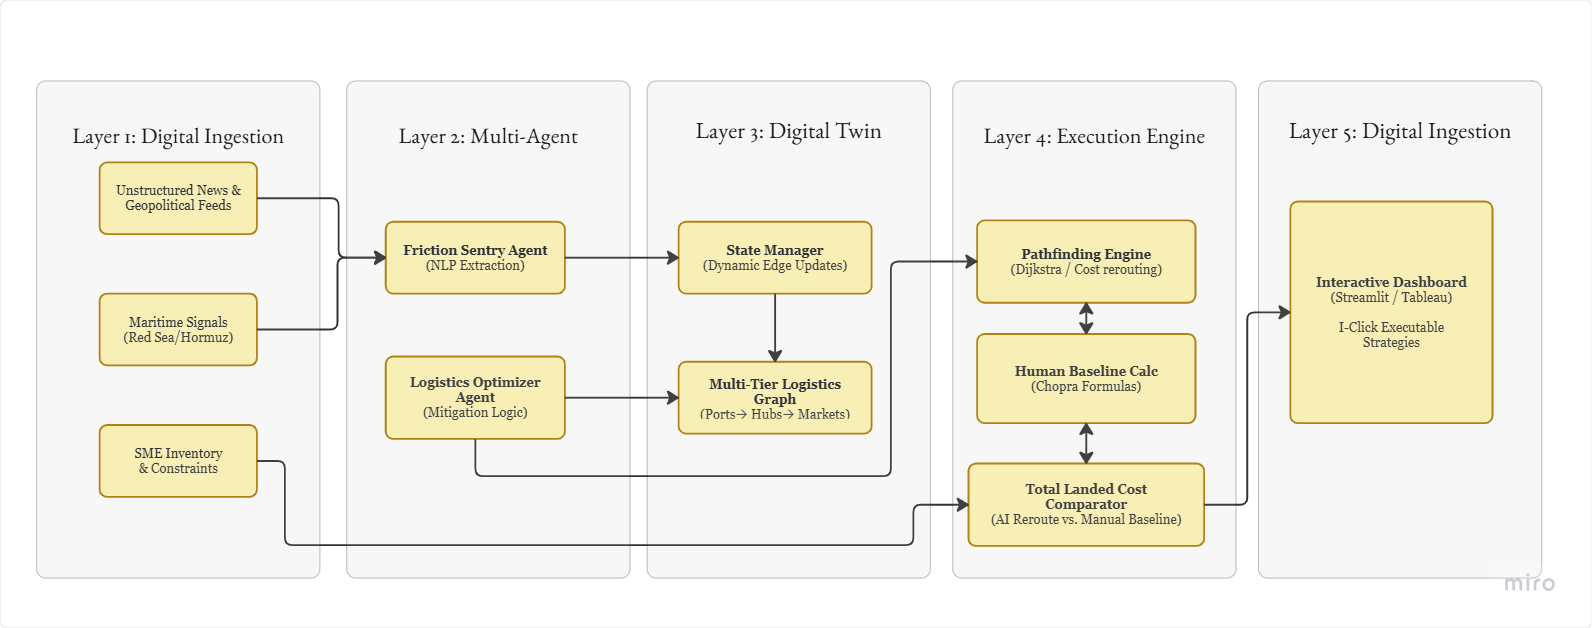
\includegraphics[width=\textwidth]{Figures/hldd.png}
    \caption{High-level design diagram of the proposed system}
    \label{fig:hldd}
\end{figure}

\subsection[Module Description]{Module Description}
This subsection provides a detailed functional breakdown of the four core modules that constitute the system architecture.

\subsubsection{Module 1: Friction Sentry (Signal Ingestion Module)}
\begin{itemize}
    \item \textbf{Purpose:} Acts as the entry gate for risk events. It ingests raw, unstructured or semi-structured disruption alerts (e.g., weather reports, blockades, news alerts) and translates them into structured, quantitative risk parameters.
    \item \textbf{Input:} Raw event inputs (event ID, location name, signal type, severity classification) and the static rule database (\texttt{semantic\_mapping\_rules.json}).
    \item \textbf{Processing Performed:}
    \begin{itemize}
        \item Analyzes the incoming signal type against predefined rule definitions.
        \item Resolves raw locations to system-valid node IDs.
        \item Calculates the direct severity multipliers and cascades the disruption to downstream nodes (ports/warehouses) using a decay factor.
        \item Assigns baseline cost impacts (\$USD/TEU) and delay overheads (days).
    \end{itemize}
    \item \textbf{Output:} A structured JSON shock event payload specifying target node ID, signal type, severity multiplier, and cascaded propagation rules.
\end{itemize}

\subsubsection{Module 2: Networked Digital Twin (Shock Simulation Module)}
\begin{itemize}
    \item \textbf{Purpose:} Simulates the real-time physical state of the supply chain network (lanes and warehouses) under the influence of the injected shocks, tracking safety stock margins and predicting stockouts.
    \item \textbf{Input:} Structured shock event payload (from Friction Sentry), baseline graph topology (\texttt{network\_topology.json}), and current inventory logs.
    \item \textbf{Processing Performed:}
    \begin{itemize}
        \item Re-calculates and inflates graph edge weights (transit times and freight costs) for all impacted routes.
        \item Executes the \textbf{Chopra Safety Stock Equation} to model the impact of lead-time variance ($\sigma_L$) on holding costs.
        \item Computes the \textbf{Days of Cover} (DoC) for affected SME markets.
        \item Evaluates stockout triggers by checking if the delayed transit days exceed the inventory buffer cover.
    \end{itemize}
    \item \textbf{Output:} An active, in-memory shocked network graph object and a live network inventory snapshot showing stock level utilization percentages and stockout flags.
\end{itemize}

\subsubsection{Module 3: Logistics Optimizer (Execution \& Rerouting Module)}
\begin{itemize}
    \item \textbf{Purpose:} Resolves shipping bottlenecks by finding mathematically optimal alternate paths and executing emergency inventory replenishments.
    \item \textbf{Input:} Shocked network graph, destination SME market parameters, and optimization strategy (minimize cost vs. minimize time).
    \item \textbf{Processing Performed:}
    \begin{itemize}
        \item Runs \textbf{Dijkstra's shortest path algorithm} on the dynamically weighted shocked graph to identify alternative paths.
        \item Orchestrates a multi-agent workflow (via \texttt{CrewAI}) where specialized agents verify route validity, compare costs, check stockout timelines, and call tools (e.g., \texttt{EmergencyRestockTool}) to inject inventory.
        \item Calculates the cost and time deltas (difference between baseline and shocked routing).
    \end{itemize}
    \item \textbf{Output:} An optimized alternate route path (e.g., Oman $\rightarrow$ Nhava Sheva $\rightarrow$ Mumbai $\rightarrow$ Bengaluru), optimized transit days, optimized landed cost, and emergency restocking orders.
\end{itemize}

\subsubsection{Module 4: Interactive Dashboard (Visualization Module)}
\begin{itemize}
    \item \textbf{Purpose:} Acts as the user interface (UI) to display telemetry, map route modifications, and present comparative performance metrics.
    \item \textbf{Input:} JSON payload from the backend API containing recommended route paths, coordinates, status messages, and cost/time delta comparisons.
    \item \textbf{Processing Performed:}
    \begin{itemize}
        \item Maps string node IDs to physical coordinates (latitude/longitude).
        \item Computes and overlays Leaflet map layers (dashed lines for baseline routes, solid colored lines for active alternate routes).
        \item Renders alerts, response latency values, and stockout statuses.
        \item Updates comparative KPIs comparing the human "Cost of Inaction" vs. the AI's optimized strategy.
    \end{itemize}
    \item \textbf{Output:} An interactive single-page web interface containing real-time map visualizations, data tables, and metrics dashboard cards.
\end{itemize}
\section[Data Flow Diagrams]{Data Flow Diagrams}
Data Flow Diagrams (DFDs) represent the movement and processing of data within the system. They illustrate how external signals are parsed, how graph states are modified, and how optimized recommendations are transmitted to the dashboard. The following subsections detail the data flow across three distinct levels of abstraction.
\subsection[Data Flow Diagram Level 0]{Data Flow Diagram Level 0(Context Diagram)}
The Context Diagram (Level 0) as shown in Figure \ref{fig:dfd0}  represents the highest-level view of the system, showing its boundaries and the primary external entities (Global Maritime Environment and SME Logistics Manager) that interact with the Agentic Logistic Network.

\begin{figure}[htbp]
    \centering
    \makebox[\textwidth][c]{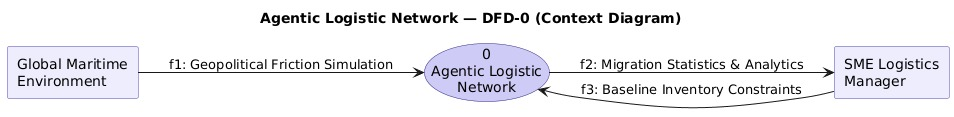
\includegraphics[width=1.15\textwidth]{Figures/DFD0.png}}
    \caption{Data Flow Diagram Level 0 (Context Diagram)}
    \label{fig:dfd0}
\end{figure}

\subsection[Data Flow Diagram Level 1]{Data Flow Diagram Level 1}
The Level 1 DFD as shown in Figure \ref{fig:dfd1} decomposes the system into its primary functional processes, illustrating the flow of data between knowledge graph construction, signal ingestion, shock propagation, and mitigation execution.

\begin{figure}[htbp]
    \centering
    \makebox[\textwidth][c]{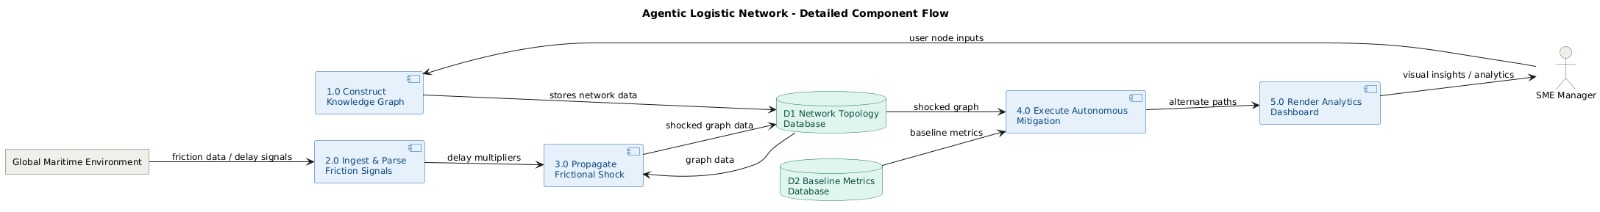
\includegraphics[width=1.26\textwidth]{Figures/DFD1.png}}
    \caption{Data Flow Diagram Level 1}
    \label{fig:dfd1}
\end{figure}

\subsection[Data Flow Diagram Level 2]{Data Flow Diagram Level 2}
The Level 2 DFD provides a granular view of the Autonomous Mitigation process (Process 4.0) as shown in Figure \ref{fig:dfd2}, detailing the sub-processes involved in identifying risks, pathfinding optimization, and strategy assembly.

\begin{figure}[htbp]
    \centering
    \makebox[\textwidth][c]{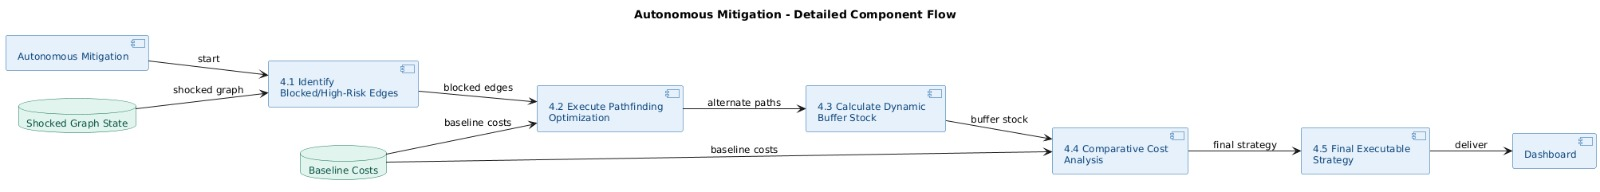
\includegraphics[width=1.26\textwidth]{Figures/DFD2.png}}
    \caption{Data Flow Diagram Level 2}
    \label{fig:dfd2}
\end{figure}

\section[UML Diagrams]{UML Diagrams}
Unified Modeling Language (UML) diagrams are presented in this section to illustrate the behavioral and structural characteristics of the system. In particular, the sequence of operations and chronological message passing between frontend, backend, and external APIs are detailed. This representation helps visualize the execution lifecycle of a simulation shock.
\subsection[Sequence Diagram]{Sequence Diagram}
The Sequence Diagram illustrated in Figure \ref{fig:sequence} shows the chronological flow of messages and operations across the system lifecycles, from initialization to final analytics delivery. The sequence begins when the \textbf{Client application (Frontend UI)} issues an execution request upon a simulated or detected chokepoint disruption. This event triggers an HTTP POST request containing location data and disruption details to the \textbf{FastAPI Web Server}. The Web Server validates the incoming payload and invokes the \textbf{Friction Sentry} module to translate the real-world textual event details into numerical severity metrics. The Friction Sentry maps the geographic location to a specific node within the logistics network topology and calculates a cascading friction multiplier based on chokepoint vulnerability tiers. Once this calculation is complete, a structured shock payload is returned to the FastAPI Web Server, which then forwards the state changes to the \textbf{Networked Digital Twin}. The Digital Twin applies these updates to its in-memory network representation, altering the travel time and shipping costs of the affected edges. Simultaneously, it evaluates the downstream impact on inventory levels, computing the Days of Cover (DoC) for the target destination markets. If the calculated DoC falls below safety thresholds, the Digital Twin alerts the Web Server, which triggers the \textbf{Logistics Optimizer} to execute routing optimization. The Optimizer queries the Digital Twin for the current state of the network graph and executes Dijkstra's pathfinding algorithm to calculate the baseline mathematically optimal path. It then forwards the computed path, inventory shortages, and node metrics to the \textbf{CrewAI Orchestrator} to initiate the agentic reasoning phase. The CrewAI Orchestrator invokes three specialized agents: the \textit{Logistics Analyst Agent}, the \textit{Logistics Optimizer Agent}, and the \textit{SME Communicator Agent}. The Analyst Agent assesses geopolitical risks and potential cascading failures; the Optimizer Agent validates the path constraints and assesses the Cost of Inaction (CoI) to determine emergency replenishment triggers; and the Communicator Agent formats these insights into a structured, actionable logistics advisory. These agents query tools (such as routing and restocking databases) and call the external \textbf{Gemini LLM} to interpret risk profiles. Once the agents reach a consensus, the final advisory is serialized as a JSON object, returned through the Web Server, and rendered on the user's \textbf{Interactive Dashboard}.

\begin{figure}[H]
    \centering
    \makebox[\textwidth][c]{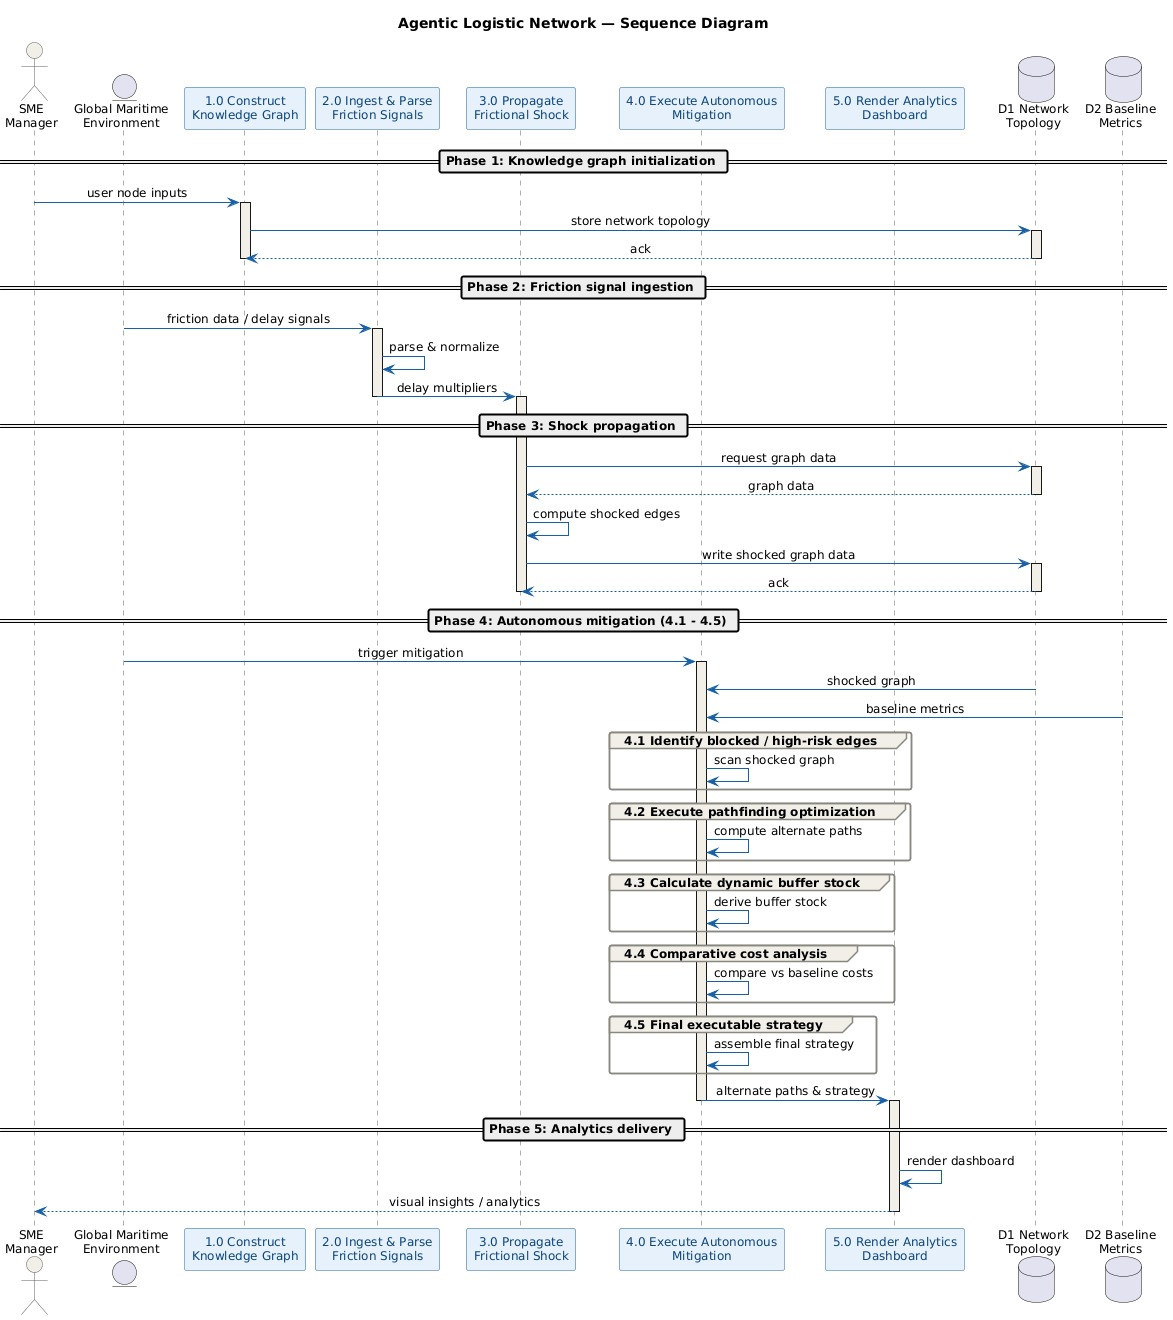
\includegraphics[width=1.1\textwidth]{Figures/sequence diagram.jpg}}
    \caption{System Sequence Diagram}
    \label{fig:sequence}
\end{figure}

\section[Summary]{Summary}
This chapter detailed the High-Level Design of the system, illustrating the modular architecture and data flow between the intelligence, optimization, and visualization layers. It established the core strategies for scalability and reliability, ensuring the framework can handle dynamic supply chain shocks effectively. The architectural blueprint provided here guides the detailed module development discussed in the next chapter.
